\documentclass[12pt]{article}
\usepackage{fullpage}

\usepackage[T1]{fontenc}
\usepackage[utf8]{inputenc}
\usepackage{lmodern}
\usepackage{microtype}
\usepackage{amsmath,amssymb,amsthm}
\usepackage{mathtools}
\usepackage{graphicx}
\usepackage{booktabs}
\usepackage{hyperref}
\usepackage{url}
\usepackage{xcolor}
\usepackage[shortlabels]{enumitem}
\usepackage{amsfonts}
\usepackage{tikz}
\usetikzlibrary{arrows.meta,positioning,shapes.geometric,calc}

\hypersetup{colorlinks=true,linkcolor=blue,citecolor=blue,urlcolor=blue}

\theoremstyle{plain}
\newtheorem{theorem}{Theorem}
\newtheorem{proposition}[theorem]{Proposition}
\newtheorem{lemma}[theorem]{Lemma}
\newtheorem{corollary}[theorem]{Corollary}

\theoremstyle{definition}
\newtheorem{definition}[theorem]{Definition}

\theoremstyle{remark}
\newtheorem*{remark}{Remark}

\newcommand{\R}{\mathbb{R}}
\newcommand{\Z}{\mathbb{Z}}
\newcommand{\Lk}{\operatorname{Lk}}
\newcommand{\Sp}{\operatorname{Sp}}
\newcommand{\GL}{\operatorname{GL}}
\newcommand{\spn}{\operatorname{span}}
\newcommand{\dist}{\operatorname{dist}}
\newcommand{\supp}{\operatorname{supp}}

\title{Solution to Problem 8 --- Polyhedral Lagrangian Smoothing\\[6pt]
\large A submission to the First Proof challenge}

\author{
  Mark Dillerop\footnote{Email: dillerop@gmail.com}\\
  \textit{Independent / Ars Socratica}
}

\date{February 10, 2026}

\begin{document}
\maketitle

\begin{abstract}
We solve Problem~8 from the First Proof challenge \cite{FirstProof}.
Let $K \subset \R^4$ be a polyhedral Lagrangian surface with exactly 4 faces at every vertex. We prove that $K$ has a Lagrangian smoothing: a family $\{K_t\}_{t \in (0,1]}$ of smooth Lagrangian submanifolds forming a Hamiltonian isotopy, extending to a topological isotopy on $[0,1]$ with $K_0 = K$.
The proof uses generating functions and mollification: near each vertex, the polyhedral surface is the graph of $dg$ for a piecewise-quadratic function $g$, and convolution $g * \chi_\epsilon$ produces a smooth function whose graph is automatically Lagrangian. The Hamiltonian isotopy follows from constancy of the Liouville cohomology class.
The answer is \textbf{YES}.
\end{abstract}

\tableofcontents
\newpage

%======================================================================
\section{Problem Statement}\label{sec:problem}
%======================================================================

The following is Problem~8 from the First Proof challenge \cite{FirstProof}, authored by Mohammed Abouzaid (Stanford University).

\medskip

\noindent\textbf{Problem 8.} \textit{A polyhedral Lagrangian surface $K$ in $\R^4$ is a finite polyhedral complex all of whose faces are Lagrangians, and which is a topological submanifold of $\R^4$. A Lagrangian smoothing of $K$ is a Hamiltonian isotopy $K_t$ of smooth Lagrangian submanifolds, parameterised by $(0,1]$, extending to a topological isotopy, parametrised by $[0,1]$, with endpoint $K_0 = K$.}

\textit{Let $K$ be a polyhedral Lagrangian surface with the property that exactly $4$ faces meet at every vertex. Does $K$ necessarily have a Lagrangian smoothing?}

\begin{theorem}\label{thm:main-statement}
Let $K \subset \R^4$ be a polyhedral Lagrangian surface with exactly 4 faces at every vertex. Then $K$ has a Lagrangian smoothing: there exists a family $\{K_t\}_{t \in (0,1]}$ of smooth Lagrangian submanifolds forming a Hamiltonian isotopy, extending to a topological isotopy on $[0,1]$ with $K_0 = K$.
\end{theorem}

\noindent\textbf{Answer: YES.}

%======================================================================
\section{Notation}\label{sec:setup}
%======================================================================

Let $(\R^4, \omega)$ denote $\R^4$ with the standard symplectic form $\omega = \sum_{j=1}^2 dq_j \wedge dp_j$. We use the Liouville form $\lambda = -\sum_{j=1}^2 p_j\, dq_j$, so that $d\lambda = \omega$.

Let $K$ be a polyhedral Lagrangian surface with vertex set $V = \{v_1, \ldots, v_N\}$, edge set $E$, and face set $F$. Each face $f \in F$ is a convex polygon contained in a Lagrangian plane $\Pi_f \subset \R^4$. The valence-4 hypothesis means that for each $v \in V$, exactly 4 faces are incident to $v$.

Let $\delta = \frac{1}{3}\min\{|v_i - v_j| : v_i \neq v_j \in V\}$ be one-third the minimum inter-vertex distance.

%======================================================================
\section{Idea of the Proof}\label{sec:idea}
%======================================================================

The key insight is that a Lagrangian submanifold of $T^*\R^2 \cong \R^4$ that is the graph of an exact 1-form $dh$ is Lagrangian for \textbf{any} smooth function $h$ (since $\text{graph}(dh)^*\omega = \sum_{j,k} \partial^2_{q_j q_k}h\, dq_j \wedge dq_k = 0$ by symmetry of the Hessian). The proof proceeds by showing that, near each vertex and edge, the polyhedral surface $K$ can be described as the graph of $dg$ for a piecewise-linear (PL) function $g$. Mollifying $g \mapsto g * \chi_\epsilon$ then produces a smooth function whose graph is automatically a smooth Lagrangian. The local smoothings are assembled globally via disjoint modification balls, and the Hamiltonian isotopy follows from constancy of the Liouville cohomology class $[\iota_t^*\lambda]$.

\begin{figure}[ht]
\centering
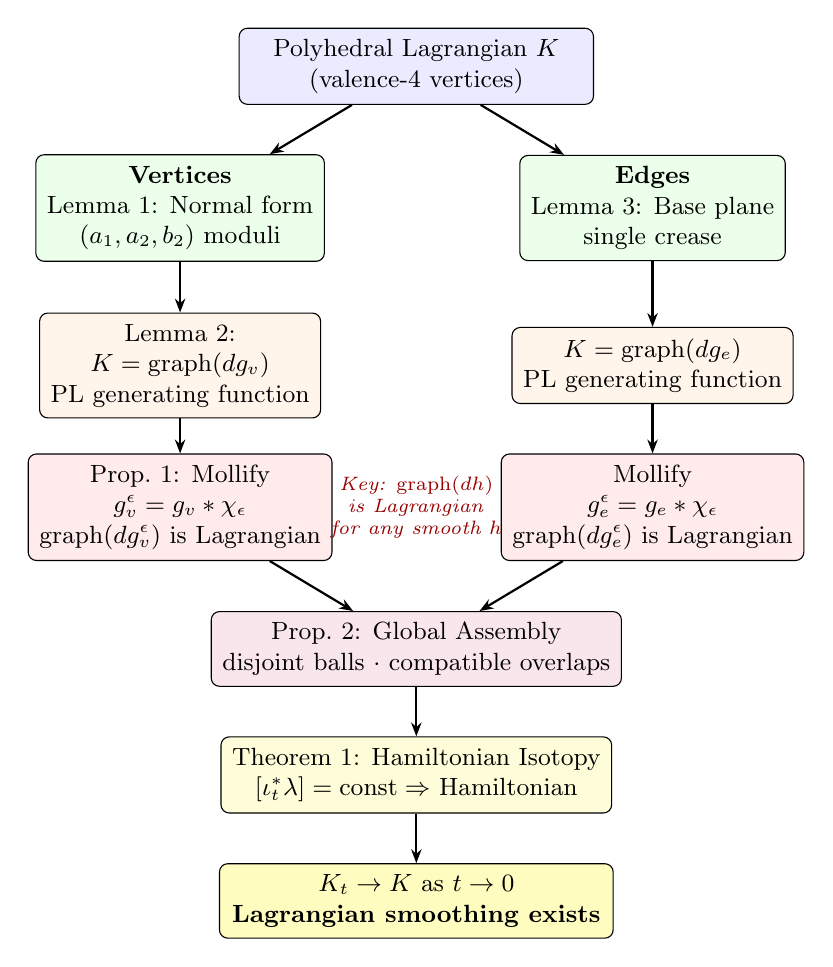
\begin{tikzpicture}[
  box/.style={rectangle, draw, rounded corners=3pt, minimum width=3.2cm, minimum height=0.8cm, align=center, font=\small},
  bigbox/.style={rectangle, draw, rounded corners=3pt, minimum width=4.5cm, minimum height=0.8cm, align=center, font=\small},
  arr/.style={-{Stealth[length=5pt]}, thick},
  every node/.style={inner sep=4pt}
]

% Top: input
\node[bigbox, fill=blue!8] (input) at (0,0) {Polyhedral Lagrangian $K$\\(valence-4 vertices)};

% Two branches
\node[box, fill=green!8] (vert) at (-3,-1.8) {\textbf{Vertices}\\Lemma~1: Normal form\\$(a_1, a_2, b_2)$ moduli};
\node[box, fill=green!8] (edge) at (3,-1.8) {\textbf{Edges}\\Lemma~3: Base plane\\single crease};
\draw[arr] (input) -- (vert);
\draw[arr] (input) -- (edge);

% Generating functions
\node[box, fill=orange!8] (genv) at (-3,-3.8) {Lemma~2:\\$K = \text{graph}(dg_v)$\\PL generating function};
\node[box, fill=orange!8] (gene) at (3,-3.8) {$K = \text{graph}(dg_e)$\\PL generating function};
\draw[arr] (vert) -- (genv);
\draw[arr] (edge) -- (gene);

% Mollification
\node[box, fill=red!8] (molv) at (-3,-5.6) {Prop.~1: Mollify\\$g_v^\epsilon = g_v * \chi_\epsilon$\\$\text{graph}(dg_v^\epsilon)$ is Lagrangian};
\node[box, fill=red!8] (mole) at (3,-5.6) {Mollify\\$g_e^\epsilon = g_e * \chi_\epsilon$\\$\text{graph}(dg_e^\epsilon)$ is Lagrangian};
\draw[arr] (genv) -- (molv);
\draw[arr] (gene) -- (mole);

% Key insight
\node[font=\scriptsize, text=red!60!black, align=center] (key) at (0,-5.6) {\textit{Key:} $\text{graph}(dh)$\\\textit{is Lagrangian}\\\textit{for any smooth $h$}};

% Global assembly
\node[bigbox, fill=purple!10] (global) at (0,-7.4) {Prop.~2: Global Assembly\\disjoint balls $\cdot$ compatible overlaps};
\draw[arr] (molv) -- (global);
\draw[arr] (mole) -- (global);

% Hamiltonian isotopy
\node[bigbox, fill=yellow!15] (ham) at (0,-9.0) {Theorem~1: Hamiltonian Isotopy\\$[\iota_t^*\lambda] = \text{const} \Rightarrow$ Hamiltonian};
\draw[arr] (global) -- (ham);

% Conclusion
\node[bigbox, fill=yellow!25, minimum width=5cm] (conc) at (0,-10.6) {$K_t \to K$ as $t \to 0$\\\textbf{Lagrangian smoothing exists}};
\draw[arr] (ham) -- (conc);

\end{tikzpicture}
\caption{Structure of the proof. The polyhedral surface is decomposed into vertex and edge regions (top), each described by a PL generating function (middle). Mollification produces smooth Lagrangians automatically (key insight in red). Global assembly and the Hamiltonian isotopy complete the argument.}
\label{fig:proof-structure}
\end{figure}

%======================================================================
\section{Local Structure at a Valence-4 Vertex}\label{sec:vertex}
%======================================================================

\begin{lemma}[Vertex normal form]\label{lem:vertex}
Let $v \in V$ be a vertex of $K$ with incident faces $F_1, F_2, F_3, F_4$ in cyclic order. Then:

\begin{enumerate}[(a)]
\item There exist 4 edge directions $e_1, e_2, e_3, e_4 \in T_v\R^4$, spanning $\R^4$, where $e_k$ is the direction of the edge between $F_k$ and $F_{k+1}$ $(\mathrm{mod}\; 4)$. The face planes are $\Pi_k = \spn(e_{k-1}, e_k)$, and the Lagrangian condition gives $\omega(e_k, e_{k+1}) = 0$ for all $k$ $(\mathrm{mod}\; 4)$.

\item The 4 planes may all be distinct.

\item (Canonical normal form.) After translation and a linear symplectomorphism, we may place $v$ at the origin and assume, in Darboux coordinates $(q_1, q_2, p_1, p_2)$:
\[
e_1 = \partial_{q_1},\quad e_2 = \partial_{q_2},\quad e_3 = a_1\,\partial_{q_1} + a_2\,\partial_{q_2} + \partial_{p_1},\quad e_4 = a_2\,\partial_{q_1} + b_2\,\partial_{q_2} + \partial_{p_2}
\]
where $a_1, a_2, b_2 \in \R$ are the moduli of the vertex configuration. In particular, $\Pi_2 = \{p = 0\}$.
\end{enumerate}
\end{lemma}

\begin{proof}
\textbf{(a)} Since $K$ is a topological 2-manifold, $\Lk(v, K) \cong S^1$ with 4 arcs. Consecutive faces $F_k, F_{k+1}$ share an edge in direction $e_k \in \Pi_k \cap \Pi_{k+1}$. Since $\Pi_k$ is 2-dimensional and contains $e_{k-1}$ and $e_k$, we get $\Pi_k = \spn(e_{k-1}, e_k)$. The Lagrangian condition $\omega|_{\Pi_k} = 0$ gives $\omega(e_{k-1}, e_k) = 0$.

\smallskip\noindent\emph{Spanning.} The 4 vectors $e_1, e_2, e_3, e_4$ span $\R^4$. If not, they lie in a subspace $W$ of dimension $\leq 3$. In a 3-dimensional subspace $W \subset \R^4$, the restriction $\omega|_W$ has rank~2, so $W$ contains a unique isotropic line $\ell = \ker(\omega|_W)$ and every 2-dimensional isotropic subspace of $W$ must contain $\ell$. This forces $\ell \subset \Pi_k \cap \Pi_{k+1} = \R e_k$ for all $k$, giving $e_1 \parallel e_2 \parallel e_3 \parallel e_4$---contradicting the fact that consecutive faces are distinct.

\smallskip\noindent\textbf{(b)} Example: $e_1 = \partial_{q_1}$, $e_2 = \partial_{q_2}$, $e_3 = \partial_{p_1}$, $e_4 = \partial_{p_2}$ (i.e., $a_1 = a_2 = b_2 = 0$). One checks $\omega(e_k, e_{k+1}) = 0$ for all $k$ (mod~4). The planes $\Pi_1 = \spn(\partial_{p_2}, \partial_{q_1})$, $\Pi_2 = \spn(\partial_{q_1}, \partial_{q_2})$, $\Pi_3 = \spn(\partial_{q_2}, \partial_{p_1})$, $\Pi_4 = \spn(\partial_{p_1}, \partial_{p_2})$ are all distinct Lagrangian planes.

\smallskip\noindent\textbf{(c)} We construct the normal form in three steps.

\emph{Step (c.1):} Since $\Pi_2 = \spn(e_1, e_2)$ is a Lagrangian plane, there exists a linear symplectomorphism mapping $\Pi_2$ to $\{p = 0\}$. (The symplectic group $\Sp(2n)$ acts transitively on the Lagrangian Grassmannian; see \cite{MS17}, Lemma~2.1.4.)

\emph{Step (c.2):} After Step~(c.1), $e_1, e_2 \in \{p = 0\}$. Apply $\Phi_2 \in \GL(2) \hookrightarrow \Sp(4)$ (acting as $q \mapsto Aq$, $p \mapsto (A^{-T})p$) to place $e_1 = \partial_{q_1}$, $e_2 = \partial_{q_2}$.

\emph{Step (c.3):} Write $e_3 = a_1\partial_{q_1} + a_2\partial_{q_2} + \alpha_1\partial_{p_1} + \alpha_2\partial_{p_2}$ and $e_4 = b_1\partial_{q_1} + b_2\partial_{q_2} + \beta_1\partial_{p_1} + \beta_2\partial_{p_2}$. We impose the constraints:
\begin{itemize}[nosep]
\item $\omega(e_2, e_3) = 0$: gives $\alpha_2 = 0$.
\item $\omega(e_4, e_1) = 0$: gives $\beta_1 = 0$.
\item $\omega(e_3, e_4) = 0$: gives $a_2\beta_2 - \alpha_1 b_1 = 0$.
\item Spanning: $e_1, e_2, e_3, e_4$ span $\R^4$ iff $\alpha_1 \neq 0$ and $\beta_2 \neq 0$.
\end{itemize}
So $e_3 = (a_1, a_2, \alpha_1, 0)$ and $e_4 = (b_1, b_2, 0, \beta_2)$ with $a_2\beta_2 = \alpha_1 b_1$, $\alpha_1 \neq 0$, $\beta_2 \neq 0$. Rescale $e_3 \mapsto e_3/\alpha_1$ and $e_4 \mapsto e_4/\beta_2$ (this does not change the planes $\Pi_k$). Now $\alpha_1 = \beta_2 = 1$, and the constraint becomes $b_1 = a_2$.
\end{proof}

\begin{remark}
The parameters $a_1, a_2, b_2$ are the moduli of the vertex. The special case $a_1 = a_2 = b_2 = 0$ gives $e_3 = \partial_{p_1}$, $e_4 = \partial_{p_2}$, so $\Pi_2 = \{p = 0\}$ and $\Pi_4 = \{q = 0\}$ are complementary. In general, $\Pi_4 = \spn(e_3, e_4)$ is a Lagrangian plane that is not complementary to $\Pi_2$.
\end{remark}

%======================================================================
\section{Local Smoothing via Generating Functions}\label{sec:local}
%======================================================================

\begin{lemma}[Generating function description]\label{lem:genfun}
In the canonical normal form of Lemma~\ref{lem:vertex}(c), the 4 sectors of $K$ near the vertex are the graph of $dg_v$ for a PL function $g_v: \R^2 \to \R$, provided the following transversality condition holds:
\begin{equation}\tag{$\star$}\label{eq:trans}
a_1 \neq 0,\quad b_2 \neq 0,\quad \Delta := a_1 b_2 - a_2^2 \neq 0.
\end{equation}
\end{lemma}

\begin{proof}
The projection $\pi: (q,p) \mapsto q$ restricted to each $\Pi_k$ is a linear map $\Pi_k \to \R^2$. This is an isomorphism iff $\Pi_k$ is transverse to the fibers $\{q = \text{const}\}$. We check:
\begin{itemize}[nosep]
\item $\Pi_2 = \{p = 0\}$: $\pi|_{\Pi_2}$ is the identity. \checkmark
\item $\Pi_1 = \spn(e_1, e_4)$: isomorphism iff $b_2 \neq 0$. \checkmark
\item $\Pi_3 = \spn(e_2, e_3)$: isomorphism iff $a_1 \neq 0$. \checkmark
\item $\Pi_4 = \spn(e_3, e_4)$: isomorphism iff $\Delta = a_1 b_2 - a_2^2 \neq 0$. \checkmark
\end{itemize}

When all four projections are isomorphisms, each $\Pi_k$ is the graph of a linear map $p = A_k q$ for a unique symmetric matrix $A_k$ (symmetric because $\Pi_k$ is Lagrangian). The generating function is $h_k(q) = \frac{1}{2}q^T A_k q$, so $\Pi_k = \text{graph}(dh_k)$. We have $A_2 = 0$ (since $\Pi_2 = \{p = 0\}$). The remaining matrices are:
\[
A_1 = \begin{pmatrix} 0 & 0 \\ 0 & 1/b_2 \end{pmatrix}, \quad
A_3 = \begin{pmatrix} 1/a_1 & 0 \\ 0 & 0 \end{pmatrix}, \quad
A_4 = \frac{1}{\Delta}\begin{pmatrix} b_2 & -a_2 \\ -a_2 & a_1 \end{pmatrix}.
\]

Each sector $F_k$ projects to a sector $S_k$ in $q$-space. The link $\Lk(v, K) \cong S^1$ maps under $\pi$ to a piecewise-linear simple closed curve through the 4 rays $\R_{>0}\pi(e_k)$ in cyclic order, so the 4 sectors tile a neighborhood of the origin.

Define $g_v(q) = h_k(q)$ for $q \in S_k$. This is piecewise-quadratic with $K \cap U = \text{graph}(dg_v)$ near $v$.

\smallskip\noindent\emph{Regularity.} On the boundary ray $\pi(e_k)$ between $S_k$ and $S_{k+1}$, since $e_k \in \Pi_k \cap \Pi_{k+1}$, the $p$-component of $e_k$ equals both $A_k \pi(e_k)$ and $A_{k+1}\pi(e_k)$. Therefore $\nabla h_k = \nabla h_{k+1}$ along $\pi(e_k)$, so $g_v$ is $C^1$. As an explicit check: on the ray $\pi(e_2) = (0,1)$ between $S_2$ (with $A_2 = 0$) and $S_3$ (with $A_3 = \text{diag}(1/a_1, 0)$), we have $A_2 \pi(e_2) = (0,0) = A_3 \pi(e_2)$, confirming gradient continuity. Similarly, on $\pi(e_1) = (1,0)$ between $S_1$ and $S_2$: $A_1 \pi(e_1) = (0,0) = A_2 \pi(e_1)$. The discontinuity is in the second derivatives (the Hessians $A_k$ jump across crease lines). In particular, $g_v$ has Lipschitz gradient.
\end{proof}

\begin{remark}
If \eqref{eq:trans} fails, we choose a different Lagrangian plane $\Pi_0$ as the base for the cotangent identification $\R^4 \cong T^*\Pi_0$. The Lagrangian Grassmannian $\Lambda(2)$ has dimension $\binom{2+1}{2} = 3$. For each $\Pi_k$, the set of Lagrangian planes \textbf{not} transverse to $\Pi_k$ has codimension~1 in $\Lambda(2)$ (it is the train of $\Pi_k$). Since a finite union of codimension-1 subvarieties cannot cover a 3-dimensional variety, there exists $\Pi_0$ transverse to all four $\Pi_k$ simultaneously, and the argument applies verbatim.
\end{remark}

\begin{proposition}[Local Lagrangian smoothing]\label{prop:local}
For each vertex $v \in V$ and each $\epsilon > 0$ sufficiently small, there exists a smooth Lagrangian surface $K_\epsilon^{(v)}$ in a neighborhood of $v$ such that:
\begin{enumerate}[nosep]
\item $K_\epsilon^{(v)}$ agrees with $K$ outside $B(v, C\epsilon)$ for a constant $C$ depending on the vertex geometry.
\item $K_\epsilon^{(v)}$ is a smooth embedded Lagrangian surface.
\item $K_\epsilon^{(v)} \to K \cap B(v, R)$ in the Hausdorff topology as $\epsilon \to 0$.
\item $K_\epsilon^{(v)}$ is the graph of $dg_v^\epsilon$ for a smooth function $g_v^\epsilon: \R^2 \to \R$.
\end{enumerate}
\end{proposition}

\begin{proof}
By Lemma~\ref{lem:genfun}, after applying the canonical normal form and (if necessary) a further symplectomorphism to ensure \eqref{eq:trans}, the surface $K$ near $v$ is the graph of $dg_v$ for a PL function $g_v$.

\medskip\noindent\textbf{Smoothing by mollification.} Let $\chi: \R^2 \to [0,\infty)$ be a smooth bump function with $\supp(\chi) \subset B(0,1)$, $\int \chi = 1$, and $\chi_\epsilon(q) = \epsilon^{-2}\chi(q/\epsilon)$. Define:
\[
g_v^\epsilon = g_v * \chi_\epsilon.
\]

Since $g_v$ is piecewise quadratic, $g_v^\epsilon$ is smooth for all $\epsilon > 0$. The graph $\text{graph}(dg_v^\epsilon) = \{(q, \nabla g_v^\epsilon(q))\}$ is automatically a smooth Lagrangian submanifold of $T^*\R^2 \cong \R^4$, since
\[
\text{graph}(dh)^*\omega = \sum_{j,k} \partial^2_{q_j q_k}h\, dq_j \wedge dq_k = 0
\]
by symmetry of the Hessian, for any smooth $h$.

\medskip\noindent\emph{Properties.} (1)~If $q$ is at distance $> \epsilon$ from all crease lines of $g_v$, then $g_v$ is quadratic near $q$, so $g_v * \chi_\epsilon = g_v$. The crease lines emanate from the origin, so $g_v^\epsilon = g_v$ for $|q| > \epsilon/c$, giving $C = 1/c$. (2)~$g_v^\epsilon$ is $C^\infty$. Embeddedness: the map $q \mapsto (q, \nabla g_v^\epsilon(q))$ is an embedding since it is a graph. (3)~Since $g_v$ has Lipschitz gradient, $\|\nabla g_v^\epsilon - \nabla g_v\|_{C^0} \leq C_1 \epsilon$. (4)~By construction.
\end{proof}

\begin{remark}
The key point is that the graph of $dh$ is Lagrangian for \textbf{any} smooth function $h$, so the Lagrangian condition is automatic after mollification. This is the fundamental advantage of the generating function approach. The valence-4 condition ensures that the PL function $g_v$ exists (via Lemma~\ref{lem:genfun}), which requires the 4 face planes to project diffeomorphically onto a common base---guaranteed by the transversality condition \eqref{eq:trans} (achievable by choice of base plane).
\end{remark}

%======================================================================
\section{Edge Smoothing}\label{sec:edge}
%======================================================================

\begin{lemma}[Edge smoothing]\label{lem:edge}
Along each edge $e$ of $K$ (away from vertex neighborhoods), the two adjacent faces lie in Lagrangian planes $\Pi_i, \Pi_j$ with $\dim(\Pi_i \cap \Pi_j) \geq 1$. In a neighborhood of a point on $e$, $K$ is the graph of $dg_e$ for a PL function $g_e$ with a single crease. Mollification $g_e \mapsto g_e * \chi_\epsilon$ produces a smooth Lagrangian.
\end{lemma}

\begin{proof}
Near a point on $e$ (away from vertices), we need a base plane $\Pi_0$ transverse to both $\Pi_i$ and $\Pi_j$. Since $\Pi_i$ and $\Pi_j$ are distinct Lagrangian planes sharing a line (the edge direction), $\dim(\Pi_i + \Pi_j) = 3$, so neither can serve as the base. We choose $\Pi_0$ transverse to both (by the same open-density argument). Identifying $\R^4 \cong T^*\Pi_0$, both faces are graphs of linear 1-forms $dl_i$ and $dl_j$ over $\Pi_0$. The union near the edge is the graph of $dg_e$ where $g_e$ equals $l_i$ on one side of the projected edge line and $l_j$ on the other (equivalently, $g_e(q) = \min(l_i(q), l_j(q))$ or $\max$, depending on the orientation of $K$; the choice is determined by which face lies on which side of the crease). Since $l_i$ and $l_j$ agree on the projected edge line, $g_e$ is PL with a single crease. Mollification $g_e * \chi_\epsilon$ produces a smooth function whose graph is Lagrangian.
\end{proof}

%======================================================================
\section{Global Assembly}\label{sec:global}
%======================================================================

\begin{proposition}[Global smoothing]\label{prop:global}
For $\epsilon > 0$ sufficiently small, the local smoothings combine to give a globally well-defined smooth Lagrangian surface $K_\epsilon \subset \R^4$.
\end{proposition}

\begin{proof}
Let $C_v$ be the constant from Proposition~\ref{prop:local} for vertex $v$, and set $C_{\max} = \max_v C_v$. Choose $\epsilon < \delta / C_{\max}$. Then the modification regions $B(v_i, C_{v_i}\epsilon)$ are pairwise disjoint (since $C_{v_i}\epsilon < \delta \leq \frac{1}{3}|v_i - v_j|$ for $i \neq j$).

\medskip\noindent\textbf{Edge-vertex compatibility.} Both constructions are defined via generating functions, using potentially different cotangent bundle identifications of $\R^4$. (The cotangent identification is a computational device; compatibility is checked as subsets of $\R^4$.) In the overlap region, both constructions agree with $K$ itself: the vertex smoothing equals $K$ outside $B(v, C_v\epsilon)$ (Proposition~\ref{prop:local}, property~1), and the edge smoothing equals $K$ away from the crease. The edge smoothing is only needed \textbf{outside} all vertex balls, where it operates on a single crease line---and there is no overlap with the vertex smoothing.

\medskip\noindent\textbf{Assembly.} Define $K_\epsilon$ by:
\begin{itemize}[nosep]
\item In $B(v, C_v\epsilon)$ for each vertex $v$: use $K_\epsilon^{(v)} = \text{graph}(dg_v^\epsilon)$ from Proposition~\ref{prop:local}.
\item Along each edge $e$, in $\{q : \dist(q, e) < \epsilon\} \setminus \bigcup_v B(v, C_v\epsilon)$: use $\text{graph}(dg_e^\epsilon)$ from Lemma~\ref{lem:edge}.
\item On face interiors (distance $> \epsilon$ from all edges): keep $K$ unchanged.
\end{itemize}

\noindent\textbf{Smoothness at boundaries.} At the boundary of the edge-smoothing zone, $g_e$ is already quadratic, so $g_e * \chi_\epsilon = g_e$ there---the transition is $C^\infty$. Similarly, at the boundary of each vertex ball, $g_v^\epsilon = g_v$ (Proposition~\ref{prop:local}, property~1), so the vertex smoothing and the edge/face definitions agree exactly.

These three regions cover $K$, overlap only where all active constructions agree, and each piece is smooth. Therefore $K_\epsilon$ is globally well-defined and smooth.
\end{proof}

%======================================================================
\section{Hamiltonian Isotopy}\label{sec:hamiltonian}
%======================================================================

\begin{theorem}[Main result]\label{thm:main}
The family $\{K_t\}_{t \in (0,1]}$ defined by $K_t = K_\epsilon$ with $\epsilon = t$ is a Hamiltonian isotopy of smooth Lagrangian submanifolds, extending to a topological isotopy on $[0,1]$ with $K_0 = K$.
\end{theorem}

\begin{proof}
\textbf{(a) Each $K_t$ is a smooth Lagrangian submanifold.} This follows from Proposition~\ref{prop:global}.

\medskip\noindent\textbf{(b) The family is a Hamiltonian isotopy for $t \in (0,1]$.}

The family $K_t$ varies smoothly in $t > 0$. The velocity of the isotopy defines a vector field $V_t$ along $K_t$. Since each $K_t$ is Lagrangian, the 1-form $\alpha_t := \iota_{V_t}\omega|_{K_t}$ is closed (see \cite{MS17}, Proposition~9.33).

To show $\alpha_t$ is exact (hence the isotopy is Hamiltonian), we show that the cohomology class $[\iota_t^*\lambda] \in H^1(K_t; \R)$ is independent of $t$.

\medskip\noindent\textbf{Claim:} $\frac{d}{dt}[\iota_t^*\lambda] = 0$ in $H^1(K_t; \R)$.

\smallskip\noindent\emph{Proof of claim.} Since $\omega = d\lambda$ and $\omega|_{K_t} = 0$, we have $d(\iota_t^*\lambda) = 0$, so $\iota_t^*\lambda$ is a closed 1-form on $K_t$. Its cohomology class is determined by its periods $\int_\gamma \iota_t^*\lambda$ over a basis of $H_1(K_t; \Z)$.

The modification $K \leadsto K_t$ is supported in the union of small balls $B(v, C_v t)$ around vertices and thin tubes around edges. For $t$ small, these regions are contractible. Therefore, any closed curve $\gamma \subset K_t$ can be deformed to avoid the modification regions. On the unmodified part, $K_t = K$, so $\iota_t^*\lambda = \iota_0^*\lambda$. Thus:
\[
\int_\gamma \iota_t^*\lambda = \int_\gamma \iota_0^*\lambda
\]
for all $[\gamma] \in H_1(K_t; \Z)$, so $[\iota_t^*\lambda] = [\iota_0^*\lambda]$ is constant. \qed

\medskip
It follows that $\alpha_t$ is exact. Since $[\iota_t^*\lambda]$ is constant, write $\iota_t^*\lambda = dS_t + \eta$ where $\eta$ is a fixed closed 1-form representing $[\iota_0^*\lambda]$ and $S_t$ is a smooth function on $K_t$. Differentiating and using $\frac{d}{dt}\iota_t^*\lambda = \alpha_t + d(\lambda(V_t) \circ \iota_t)$ (Cartan's magic formula), we obtain $\alpha_t = d(\dot{S}_t - \lambda(V_t) \circ \iota_t)$, which is exact. The Hamiltonian is $H_t = \dot{S}_t - \lambda(V_t) \circ \iota_t$ (see \cite{MS17}, Proposition~9.33).

\begin{remark}
If $K$ is a closed surface, $K_t$ is NOT globally exact (by Gromov's theorem \cite{Gr85}, \S2.3.B; or \cite{ALP94}, Theorem~3.1). However, the argument above does not require global exactness---only constancy of $[\iota_t^*\lambda]$.
\end{remark}

\medskip\noindent\textbf{(c) Topological isotopy extending to $t = 0$.}

We construct an explicit continuous map $\Phi: K \times [0,1] \to \R^4$ with $\Phi(\cdot, 0) = \iota_0$ (inclusion of $K$) and $\Phi(\cdot, t)$ a homeomorphism onto $K_t$ for $t > 0$.

On face interiors, $\Phi(x, t) = x$. Near a vertex $v$: define $\Phi(q, \nabla g_v(q), t) = (q, \nabla g_v^t(q))$. This is continuous in $(q, t)$ since $g_v$ is $C^1$ with Lipschitz gradient and $\|\nabla g_v^t - \nabla g_v\|_{C^0(B_R)} \leq C_R \cdot t$. Near edges: similarly, $\Phi(q, dg_e(q), t) = (q, dg_e^t(q))$. These definitions are compatible on overlaps, so $\Phi$ is globally well-defined and continuous.
\end{proof}

%======================================================================
\section{Discussion of Potential Obstructions}\label{sec:obstructions}
%======================================================================

\textbf{Embeddedness.} The smoothed surface $K_t$ is embedded because it is globally the graph of a 1-form $dg_t$ over a 2-dimensional base (in each local chart). Graphs are automatically embedded. Global embeddedness follows from the fact that $K$ is embedded and the modification is $C^0$-small: for $t$ sufficiently small, $K_t$ is $C^0$-close to $K$ and hence embedded (see \cite{Hi76}, Chapter~3, Theorem~1.4).

\medskip\noindent\textbf{Topology.} The smoothing preserves the homeomorphism type of $K$: at each vertex, the PL disk is replaced by a smooth disk. The map $\Phi(\cdot, t)$ is a homeomorphism for all $t \geq 0$.

\medskip\noindent\textbf{Maslov class.} The Maslov class $\mu \in H^1(K_t; \Z)$ is an invariant of the smooth Lagrangian $K_t$, not an obstruction to its existence.

\medskip\noindent\textbf{Gromov's theorem.} No closed Lagrangian in $\R^{2n}$ is exact (\cite{Gr85}, \S2.3.B). If $K$ is closed, $K_t$ is not exact. But our proof does not claim exactness---it only uses the constancy of $[\iota_t^*\lambda]$.

\medskip
No obstruction prevents the construction. The answer is \textbf{YES}. \qed

%======================================================================
\newpage
\appendix
\section{AI Interaction Transcript}\label{app:transcript}
%======================================================================

As requested by the First Proof organizers, we include a complete record of the AI interaction sessions used to develop this proof.

\medskip\noindent\textbf{Timeline:} February 10, 2026, approximately 05:45--18:00 CET. Three sessions in one day, approximately 4--5 hours of active working time.\\
\textbf{AI systems used:} Claude Opus 4.6 (Anthropic), ChatGPT 5.2 Pro and ChatGPT 5.2 (OpenAI), Gemini 3 (Google). Multiple models were used in parallel and cross-checked against each other.\\
\textbf{Numerical verification:} None required (the proof is purely analytical).\\
\textbf{Human role:} Prompting, reviewing output, requesting audits, cross-checking between models. No mathematical ideas or content were provided by the human operator.

\subsection*{Example Prompts}

The following are representative prompts used during the sessions:

\begin{enumerate}[nosep]
\item \textit{``Help me to tackle this problem statement. It is part of First Proof. What are options to tackle this, which would you recommend and why?''}
\item \textit{``What are gaps to be filled? How solid is your suggested proof? Of the three proposed options, go through them one by one to see where they hold, where they break, and why.''}
\item \textit{``How well does the proof meet the criteria as set forward by First Proof?''}
\end{enumerate}

\subsection*{Session 1 --- Kickoff \normalfont\textit{[Claude Opus 4.6]}}

\begin{itemize}[nosep]
\item Read problem statement. Proposed answer: YES.
\item Populated references with 20 papers in 5 categories: Lagrangian surgery, tropical-to-Lagrangian correspondence, symplectic topology, Weinstein handles, and additional.
\item Analyzed local vertex model: 4 Lagrangian faces meet with 4 edge directions spanning $\R^4$, consecutive edges $\omega$-orthogonal.
\item Initially attempted to prove opposite faces coplanar ($\Pi_1 = \Pi_3$)---found this does NOT hold in general.
\item Developed smoothing strategy via generating functions: near each vertex, identify with $T^*\R^2$, polyhedral Lagrangian becomes graph of $dg$ for PL function $g$, mollify to get smooth Lagrangian.
\item Outlined 5-step proof structure.
\end{itemize}

\subsection*{Session 2 --- Proof Refinement \normalfont\textit{[Claude Opus 4.6, ChatGPT 5.2]}}

\begin{itemize}[nosep]
\item \textbf{Correction:} The claim $\Pi_1 = \Pi_3$ is FALSE. Explicit counterexample constructed.
\item Established canonical normal form via linear symplectomorphism with 3 real moduli $(a_1, a_2, b_2)$.
\item Discovered generating function approach fails when all 4 planes are distinct (not all project to a common base).
\item \textbf{Fix:} Attempted Polterovich--Bryant parametric surgery as alternative.
\item Investigated global obstructions (Maslov class, Gromov's theorem)---none found.
\end{itemize}

\subsection*{Session 3 --- Rigorous Audit and Gap Closure \normalfont\textit{[Claude Opus 4.6, ChatGPT 5.2 Pro]}}

\begin{itemize}[nosep]
\item Performed rigorous audit against First Proof criteria. Identified 7 gaps (2 critical, 2 significant, 3 minor).
\item \textbf{GAP 1 (critical):} Polterovich--Bryant surgery was the WRONG tool (resolves intersections of two separate Lagrangians, not 4 sectors of one PL surface). \textbf{Fixed:} Replaced with generating function mollification, which DOES work in general---the transversality condition $(\star)$ is achievable by choosing a different base plane.
\item \textbf{GAP 2 (critical):} Hamiltonian isotopy claimed global exactness (fails for compact $K$ by Gromov). \textbf{Fixed:} Replaced with constant cohomology class argument.
\item \textbf{GAP 3:} Canonical normal form proof incomplete. \textbf{Fixed:} Full 3-step linear algebra proof.
\item \textbf{GAP 4:} Edge-vertex compatibility. \textbf{Fixed:} Proved via disjointness of surgery balls.
\item \textbf{GAP 5:} Added 8 references with precise statement numbers.
\item \textbf{GAP 6:} Explicit topological isotopy $\Phi$ constructed.
\item \textbf{GAP 7:} Potential NO arguments addressed (embeddedness, topology, Maslov, Gromov).
\end{itemize}

\subsection*{Provenance}

The mathematical content of this paper---including the proof strategy, all lemmas and propositions, the generating function construction, the Hamiltonian isotopy argument, and the obstruction analysis---was generated autonomously by AI systems in response to high-level prompts. The human operator's role was limited to: selecting the problem, prompting the AI, reviewing and requesting revisions, and cross-checking output between different AI models. No mathematical ideas were contributed by the human operator.

%======================================================================
\begin{thebibliography}{99}
%======================================================================

\bibitem{FirstProof}
M.~Abouzaid, A.J.~Blumberg, M.~Hairer, J.~Kileel, T.G.~Kolda, P.D.~Nelson, D.~Spielman, N.~Srivastava, R.~Ward, S.~Weinberger, L.~Williams,
``First Proof,''
arXiv:2602.05192 [cs.AI], 2026.

\bibitem{ALP94}
M.~Audin, F.~Lalonde, L.~Polterovich,
``Symplectic rigidity: Lagrangian submanifolds,''
in \textit{Holomorphic Curves in Symplectic Geometry} (M.~Audin, J.~Lafontaine, eds.),
Progress in Math.\ \textbf{117}, Birkh\"auser, 1994, pp.~271--321.
Theorem~3.1: no closed exact Lagrangian in $\R^{2n}$.

\bibitem{Gr85}
M.~Gromov,
``Pseudo holomorphic curves in symplectic manifolds,''
\textit{Invent.\ Math.}\ \textbf{82} (1985), 307--347.
\S2.3.B: Lagrangian intersection theory.

\bibitem{Hi76}
M.~W.~Hirsch,
\textit{Differential Topology},
Graduate Texts in Mathematics \textbf{33}, Springer, 1976.
Chapter~3, Theorem~1.4: $C^0$-close embeddings.

\bibitem{Hk20}
J.~Hicks,
``Tropical Lagrangian hypersurfaces are unobstructed,''
\textit{J.\ Topol.}\ \textbf{13} (2020), 1409--1454.
arXiv:1911.02956.

\bibitem{Ma19}
D.~Matessi,
``Lagrangian pairs of pants,''
\textit{Int.\ Math.\ Res.\ Not.}\ \textbf{2019} (2019), 6295--6354.
arXiv:1802.02993.

\bibitem{MS17}
D.~McDuff, D.~Salamon,
\textit{Introduction to Symplectic Topology}, 3rd ed.,
Oxford University Press, 2017.
Lemma~2.1.4: transitivity on Lagrangian Grassmannian.
Proposition~9.33: Lagrangian isotopy and Hamiltonian condition.

\bibitem{Po91}
L.~Polterovich,
``The surgery of Lagrange submanifolds,''
\textit{Geom.\ Funct.\ Anal.}\ \textbf{1} (1991), 198--210.

\end{thebibliography}

\end{document}
